\cleardoublepage
\backmatter
\chapter{中德文化补充说明}
    在这里我们将通过服饰、饮食、体育、工作、交通、艺术和卫生这七个角度,探索中德两国的文化差异,
领略两国各异的
人文风情和生活方式。

\section{服饰}
    传统服饰是反应过去时代文化和人们对地域环境影响下形成的文化标志之一。在历史的长河中,
各个地域、各个民族都形成了风格迥异的传统服装。在人类近代化的发展潮流中,政治、经济、文化都发生了日新月异的变化,
这些变化都会对服装的演变产生深刻的影响。如果我们仔细观察中德两国传统服饰现代化演变的过程,可以发现这样一个显著的特征,
传统服饰由原来的拘谨、保守、呆板,逐渐向美观、适体、方便、平民化转变。在这里,我将以中徳两国具有代表性的女性传统服装为例,
通过介绍它们在近代化过程中的演变,来体现两国在服装上面迥异的文化。

\subsection{旗袍的前身——旗装}
\begin{figure}[htb]
\centering
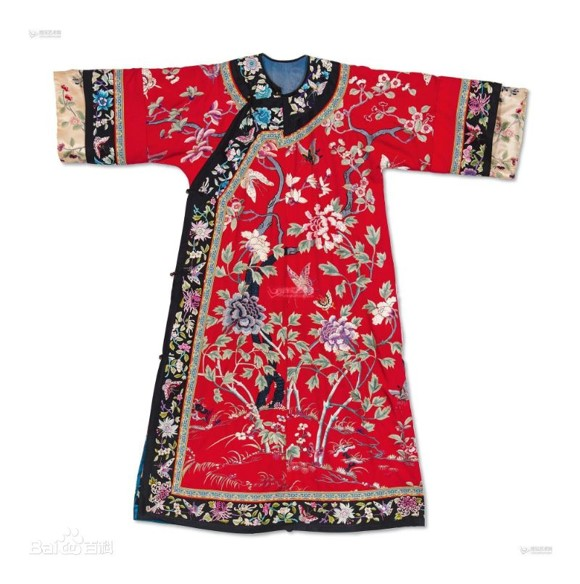
\includegraphics[width=0.6\linewidth]{Qizhuang}
\caption{清代旗装}
\end{figure}

    对于旗袍的来源,历来都有许多争议,比较主流的观点是现代旗袍改良自清代旗装。在浓厚的清朝封建礼教氛围中,妇女不可能如图现代一般将身体的曲线表现出来,否则会被视为不符合道德。因此清代旗装的裁制一直采用直线,衣身宽松,使女性身体的曲线不能外露,在现在看来,有点笨重和土气。 

    在色彩搭配方面,旗装色彩鲜艳复杂,喜欢使用高对比度的色彩搭配,并在衣身上绣有花、鸟、兽等图案,寓意吉祥,其中黄色是皇家专用的颜色,平民是禁止使用的。 
    
\subsection{旗袍的发展与流行}
\begin{figure}[htb]
\centering
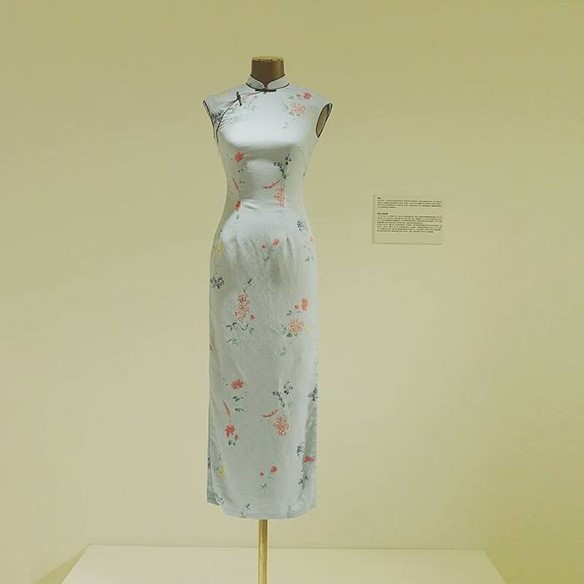
\includegraphics[width=0.6\linewidth]{Qipao}
\caption{现代旗袍}
\end{figure}

    1840年后进入近代,西洋文化侵袭着清朝的本土文化,服装也在开始发生变革。流行于二十世纪20年代的旗袍,是在民国妇女在穿着中吸收西洋服装对的式样,由传统的中国袍服不断改进而定型的。当时并没有专业服装设计机构,所以人民的服饰式样各不相同,在时代风尚的影响下不断变化。 

    从20世纪20年代至40年代末,中国旗袍风行了20多年,款式几经变化,领口的设计吸收了西式的特点,采用了当时时髦的样式,袖子也有原来的长袖改为了短袖,衣身变得更适体了,这时旗袍造型纤长,与欧洲流行的女装轮廓相吻合,让女性的体态和曲线美充分地体现出来了。 

\subsection{旗袍背后的文化内涵}

    旗袍的发展充分体现了当时妇女勇敢寻求思想上的解放,争取平等权利,反抗来自封建礼教的压迫,追寻独立自主的进步思想 。旗袍的发展历史不仅是中国服饰史的的一部分,也是中国近代化的一个标识之一。

    同样的,来自德国的传统女性服装Dirndl(德式连衣裙)也经过了一系列的改良和发展,至今仍然保留着旺盛的生命力。

\subsection{德式连衣裙的前身}
\begin{figure}[htb]
    \centering
    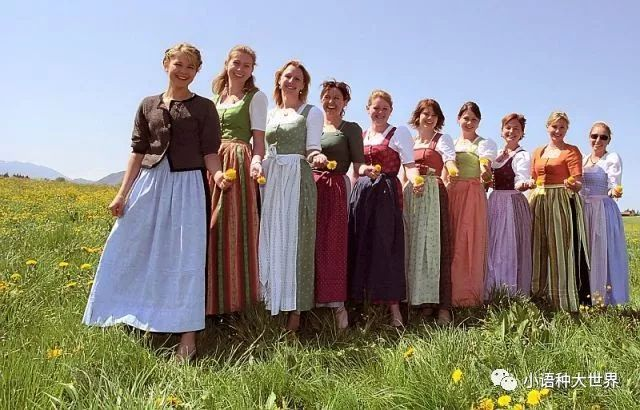
\includegraphics[width=0.6\linewidth]{alter Dirndl}
    \caption{老式Dirndl}
\end{figure}

    Dirndl是德国巴伐利亚地区和奥地利的一种传统的女性裙装。“Dirndl”原义指的是年轻姑娘,如今则为这类女性传统裙装统称。Dirndl起源于劳动妇女的工作服,材料为棉、亚麻、真丝或羊绒,颜色朴素沉静。 

    一套完整的Dirndl由四部分组成,Dirndl一般由这几个部分组成:衬衣或衬裙、紧身马甲、高腰半身裙和围裙。以前的衬衣的袖子一般都会长至肘部,“密封性"也相对较高——通常为方领或弧型领,也有长至脖子下方的,传统的半身裙也长至脚踝。 

\subsection{德式连衣裙的流行与发展}  
\begin{figure}[htb]
    \centering
    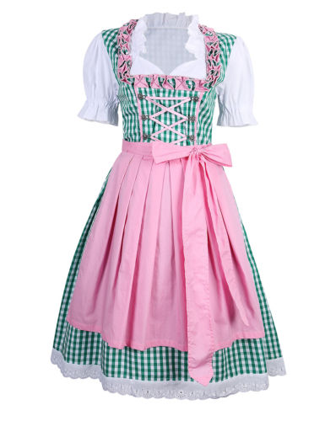
\includegraphics[width=0.6\linewidth]{neuer Dirndl}
    \caption{现代Dirndl}
\end{figure}

    随着时间的推移,服饰的发展总是趋于多元化,变得更加开放与活泼。十九世纪七八十年代的时候,城市的上流社会中有那么一群酷爱清凉一夏的人,这种轻便的田园夏装在她们之间得以流行。在一战后的经济困难时期,Dirdln彻底火了起来。因为比起那些做工精细、奢华昂贵的传统女性服装,它朴实无华又价格低廉,满足了那时广大女性的需求。

    在德意志第三帝国时期,纳粹执政党特别推崇德国传统服装。Gertrud Pesendorfer反对天主教的保守,主张在传统价值观念的框架里进行传统服饰的创新。Pesendorfer宣称,要将德国传统服饰从外来时尚艺术的影响中解放出来而使传统文化的根本重现时尚舞台。在这种情况下,Dirndl的袖子变得越来越短,衣领也变得越来越大,裙子也比原来变短了,Dirndl逐渐朝着现代服饰的方向演变。 

    如今,主要在德国南部和一些阿尔卑斯山地区,每逢集市、乡村地区的教堂落成典礼纪念日的年市或是盛大的民族节日人们还会穿着这种传统服饰。比如在盛大的慕尼黑十月啤酒节上,女士会穿上上鲜艳的Dirndl,胸前的设计突出了德国女人丰满的身材,腰间系的围裙又体现出德国女人窈窕的曲线,短短的泡泡袖设计在注重漂亮的同时,也很实用。 

\subsection{德式连衣裙上的文化内涵}  
     围裙,这块布真是充分显示出巴伐利亚妇女吃苦耐劳的品质,在十九世纪,奥地利人可是将之称为Dirndlgewand(女仆装扮)。不过,这块布可不仅仅是为了劳动而存在,它还包含着各式各样的个人信息,这在保守的时代可是相当重要:比如,围裙在左边打结,说明这位女性仍单身,当地有这样的说法:“Schleife links, Glück bringt’s!(左边系结,幸运到来)”。这样一来,单身男性就很容易分辨哪位窈窕淑女可以多加关注并有机会追求了。围裙在右面打结,表示这位女性已名花有主了。如果围裙结系在中间,说明这位女性的个人状况不确定(如下几种可能都有:处女、因为家庭原因而无法作出决定,或是自己想不清楚正在左右摇摆……)。如果围裙在身后打结,则只有两种可能:服务员或丧偶。 

\subsection{结语}  
    通过以上介绍,想必你们一定对旗袍和德式连衣裙有了基本的认识。旗袍和德式连衣裙既随着时代的发展不断变化,也保留了自己的传统和民族的特质,它们是新、旧时代交替的缩影。



\section{饮食}
     饮食文化涉及到食源的开发与利用、食具的运用与创新、食品的生产与消费、餐饮的服务与接待、餐饮业与食品业的经营与管理,以及饮食与国泰民安、饮食与文学艺术、饮食与人生境界的关系等,深厚广博。其具有风味多样,四季有别,注重情趣等特点。对于每一个学生来说,来到一个陌生的国家,饮食问题是非常重要的。为了帮助中德学子了解两国饮食文化,本文主要根据常见的饮食习俗来介绍。

\subsection{饮食文化简介}
    饮食本是人类最基本的活动,但若将问题提到为什么吃、怎么吃的层次,它就体现为一种意识或观念了。在饮食观念上,中西方有着明显的差异。

\subsection{中德——饮食文化}
    西方是一种理性的、讲求科学的饮食观念。他们强调饮食的营养价值,注重食物所含蛋白质、脂肪、热量和维生素的多少,而不追求食物的色、香、味、形的完美。 

    中国人的饮食强调感性和艺术性,追求饮食的口味感觉,而不注意食物的营养成份,多从“色、香、味、形、器”等方面来评价饮食的好坏优劣,追求的是一种难以言传的意境。简单地说,中国人吃的是口味。“味”,是中国饮食的魅力所在。中国人饮食的目的,除了果腹充饥,同时还满足对美味的渴望,带来身心的愉悦。

\subsection{中国的饮食习俗}
    中国人的饮食强调感性和艺术性,追求饮食的口味感觉,多从“色、香、味、形、器”等方面来评价饮食的好坏优劣,追求的是一种难以言传的意境。简单地说,中国人吃的是口味。“味”,是中国饮食的魅力所在。中国人饮食的目的,除了果腹充饥,同时还满足对美味的渴望,带来身心的愉悦。

\subsection{传统的中国美术——艺术}
    中国在追求食物的口味的同时,也追求食物的美感。通常会把食物雕刻成龙凤等动物的形状,或者仙桃,花朵等果实的形状。

    对食材的雕刻在中国是一门艺术,它有着自己的重要含义。龙和凤凰在中国代表着吉祥如意,而仙桃等代表着长寿。 

    长寿面是中国饮食文化的一种典型代表食物。老人在过生日时会吃这种面条,一碗面就一根面条,但是这根面条非常长,代表着祝福老人长命百岁。 

    \begin{figure}[htb]
        \centering
        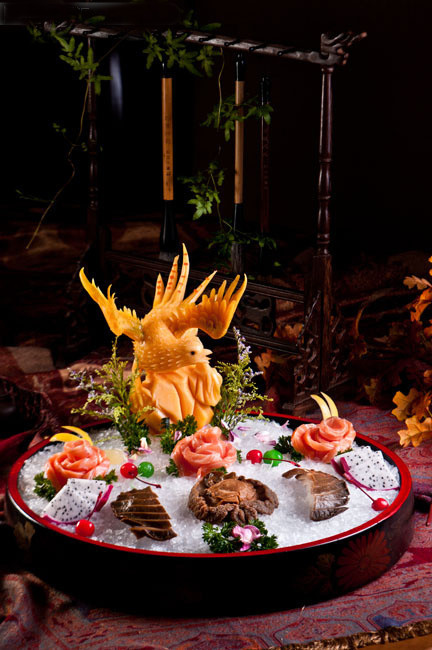
\includegraphics[width=0.6\linewidth]{caidiao}
        \caption{菜品雕刻}
    \end{figure}

\subsection{中国餐厅的饮食文化}
\item 中国餐厅是没有小费的。 
\item 一般用餐开始时间:17点到21点,持续1-2小时。 
\item 喝不重要,餐前一般会提高免费的茶水。 
\item 所有菜肴都很多。 
\item 用餐是使用筷子。 
\item 没有盐和胡椒调味。

\begin{figure}[htb]
    \centering
    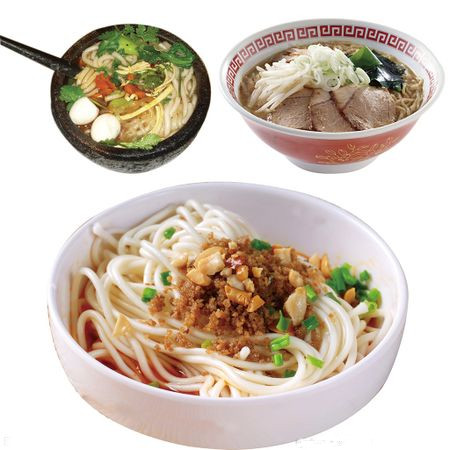
\includegraphics[width=0.6\linewidth]{noodle}
    \caption{面食}
\end{figure}

\subsection{德国的饮食习俗}
    西方是一种理性的、讲求科学的饮食观念。他们强调饮食的营养价值,注重食物所含蛋白质、脂肪、热量和维生素的多少,而不追求食物的色、香、味、形的完美。

\subsection{德国——圣诞节美食}
    下面以德国的圣诞节为例。在圣诞节时,德国人经常吃土豆沙拉,家禽或香肠。

    \begin{figure}[htb]
        \centering
        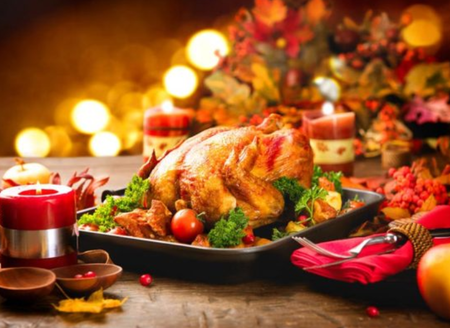
\includegraphics[width=0.6\linewidth]{christmas}
        \caption{圣诞美食}
    \end{figure}  

\subsection{德国——耶稣受难日}
    耶稣受难日德国人的食物是鱼或清淡的素食。 

    \begin{figure}[htb]
        \centering
        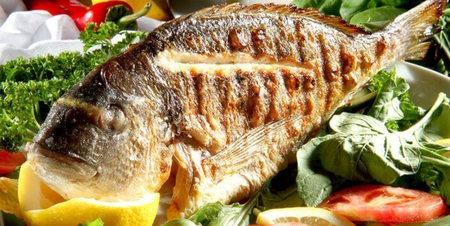
\includegraphics[width=0.6\linewidth]{fish}
        \caption{鱼}
    \end{figure}  

\subsection{德国——餐厅饮食文化}

\item 小费总额的2€至10% 
\item 开始吃饭的会议:19-20小时,2-3小时 
\item 喝重要 
\item 每个人都下令自己的法庭 
\item 餐具 
\item 调味盐和胡椒调味。

\begin{figure}[htb]
    \centering
    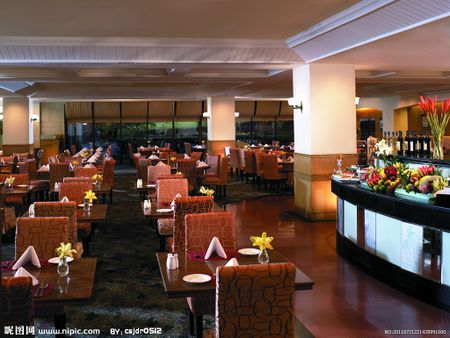
\includegraphics[width=0.6\linewidth]{restaurant}
    \caption{德国餐厅}
\end{figure} 
